\documentclass[mathserif]{beamer}

\usepackage[utf8]{inputenc} 
\usepackage[T1]{fontenc}
\usepackage{lmodern}
\usepackage{graphicx}
\usepackage[english]{babel}

\usepackage{xcolor,colortbl}

\usepackage{tikz}
\usetikzlibrary{arrows}

\usepackage{float}
\usepackage{caption}
\usepackage{subcaption}

\usetheme{Frankfurt}

\title[Defense]{IRESI - SketchMin algorithm}

\author{Simon Bihel, Florestan De Moor}
\institute[ENS Rennes]{
\includegraphics[width=3cm]{Logo_ENS_Rennes_Mention_NormaleSup}}
\date{November 25th, 2015}



\begin{document}

\section*{Introduction}

	\begin{frame}
		\maketitle
	\end{frame}
	

	
	\begin{frame}{Outline}
		\tableofcontents
	\end{frame}
	
	
\section{DDoS}

	\begin{frame}{Outline}
		\tableofcontents[currentsection]
	\end{frame}

	\subsection{Simple view}
	
	\begin{frame}{Simple attack}
	
\begin{block}

\begin{center}
\begin{tikzpicture}[->,>=stealth',shorten >=1pt,auto,node distance=4.cm]

  \node (A){
\includegraphics[scale=0.2]{computer.png}};
  \node (B) [right of=A] {
\includegraphics[scale=0.1]{router.png}};
  \node (C) [right of=B] {
\includegraphics[scale=0.2]{server.png}};

  \path
(A) edge [draw=red, line width=0.5mm] node {Packets} (B)
(B) edge [draw=purple, line width=0.5mm] node {} (C);

\end{tikzpicture}
\end{center}

\end{block}
	
	\end{frame}
	
	\subsection{Multiple streams}
	
	\begin{frame}{DDoS attack}
	
\begin{block}

\begin{center}
\begin{tikzpicture}[->,>=stealth',shorten >=1pt,auto]

\node (A){
\includegraphics[scale=0.2]{computer.png}};
\node (B) [right of=A, node distance=4.cm] {
\includegraphics[scale=0.1]{router.png}};
\node (C) [right of=B, node distance=4.cm] {
\includegraphics[scale=0.2]{server.png}};
\node (D) [below of=A, node distance=2.3cm]{
\includegraphics[scale=0.2]{computer.png}};
\node (E) [above of=A, node distance=2.3cm]{
\includegraphics[scale=0.2]{computer.png}};

  \path
(A) edge [draw=red, line width=0.5mm] node {Packets} (B)
(D) edge [draw=red, line width=0.5mm] node {Packets} (B)
(E) edge [draw=red, line width=0.5mm] node {Packets} (B)
(B) edge [draw=purple, line width=1.5mm] node {} (C);

\end{tikzpicture}
\end{center}

\end{block}
	
	\end{frame}
	
	\begin{frame}{Computing a correlation indicator}
	
	\begin{center}
		\textbf{2 DATA STREAMS}
	\end{center}
	
	\begin{center}\begin{tabular}{|c|c|c|c|c|c|c|c|c|c|c|c|c|c|c|c|c|c|c|c|}
	\hline
	~ & ~ & \cellcolor{purple}~ & ~ & \cellcolor{purple}~ & ~ & ~ & \cellcolor{purple}~ & ~ & ~ & \cellcolor{purple}~ & ~ & ~ & ~ & ~ & ~ & ~ &\cellcolor{purple}~ & ~ & ~ \\
	\hline
	\end{tabular}\end{center}
	
	\begin{center}\begin{tabular}{|c|c|c|c|c|c|c|c|c|c|c|c|c|c|c|c|c|c|c|c|}
	\hline
	\cellcolor{purple}~ & ~ & ~ & ~ & \cellcolor{purple}~ & ~ & \cellcolor{purple}~ & ~ & ~ & ~ & \cellcolor{purple}~ & ~ & ~ & ~ & \cellcolor{purple}~ & ~ & ~ & ~ & \cellcolor{purple}~ & ~ \\
	\hline
	\end{tabular}\end{center}
	
	\begin{alertblock}{Codeviance $\longrightarrow$ \texttt{if} High correlation \texttt{then} DDoS attack ongoing}
	\end{alertblock}
	
	
	\end{frame}
	

\section{Programming the algorithm}

	\begin{frame}{Outline}
		\tableofcontents[currentsection]
	\end{frame}

	\subsection{Extraction}
	
	\begin{frame}{Extraction on data traces}
		% choosed python cause of its fast development time, also the more convenient based on the languages we know
		% explain how we extract and transform them into entries to the algorithm ?
		% numpy/matplotlib ?
		\begin{block}{}
			\begin{itemize}
				\item Pick an entry on each line (=request), like the source or file requested ;
				\item convert them to integers using an injective function ;
				\item if multiple traces, extract all at once to keep correlation.
			\end{itemize}
		\end{block}
	\end{frame}
	
	\subsection{Computing the codeviance}
	
	\begin{frame}{Hashing functions}
	
	\begin{block}{}
	The data trace has integers values which stand between $0$ and $u$. We have to define $t$ universal hashing functions $h_i$ :
	\[ h_i(x) = ((a_ix+b_i) \mod u) \mod k \quad \forall i \in \lbrace 1 \ldots t \rbrace \]
where $a_i, b_i$ are randomly generated in $\lbrace 1 \dots t-1 \rbrace$ for $a_i$, and $\lbrace 0 \ldots t-1 \rbrace$ for $b_i$
	\end{block}
	
	\end{frame}
	
	\begin{frame}{Hashing functions}
	
	\begin{exampleblock}{Example}
	We generated a random data trace of size $10~000$, in $\left[0, u = 100\right]$ following a law of Poisson ($\lambda = u/2^4$). With $t=7$, $k=20$, $a=6$, $b=2$, here is the result :
	
	\begin{center}
	\begin{tabular}{cc}
		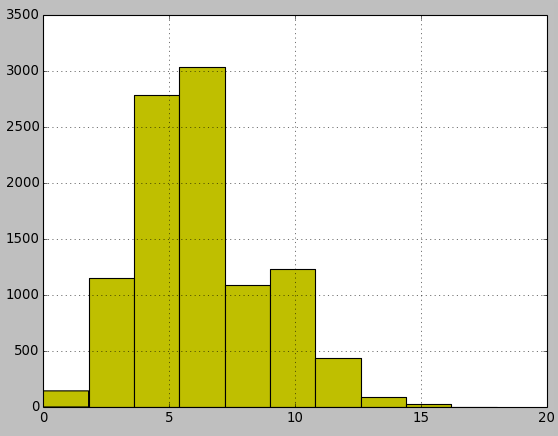
\includegraphics[scale=0.25]{poisson4.png} &
		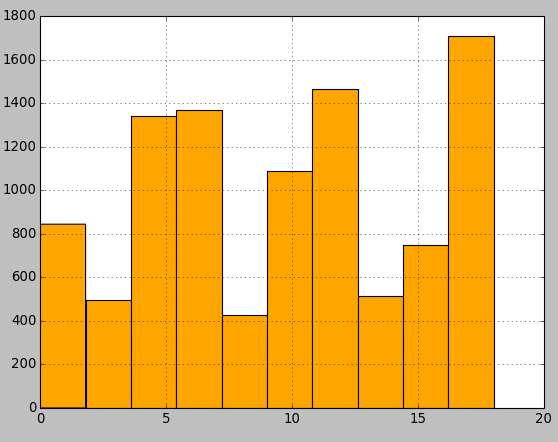
\includegraphics[scale=0.25]{poisson4_hashed.png} \\
		Raw data trace & Hashed data trace \\
	\end{tabular}
	\end{center}
	
	\end{exampleblock}

	\end{frame}
	
	\begin{frame}{Using Python 3 language}
	
	\begin{center}
		\begin{tikzpicture}[-,>=stealth',shorten >=1pt,auto]

	\node (A) {
\includegraphics[scale=0.4]{python.png}};
	\node (B) [above left of=A, node distance=3.5cm] {\begin{tabular}{|c|}\hline \texttt{Matplotlib}, \texttt{Numpy}\\ \hline \end{tabular}};
	\node (C) [above right of=A, node distance=3.5cm] {\begin{tabular}{|c|}\hline Reading files\\ \hline \end{tabular}};
	\node (D) [below left of=A, node distance=3.5cm] {\begin{tabular}{|c|}\hline Easy syntax\\ \hline \end{tabular}};
	\node (E) [below right of=A, node distance=3.5cm]{\begin{tabular}{|c|}\hline Library modules written in C\\ \hline \end{tabular}};

	\path
	
	(B) edge [draw=yellow, line width=0.5mm] node {} (A)
	(C) edge [draw=yellow, line width=0.5mm] node {} (A)
	(D) edge [draw=yellow, line width=0.5mm] node {} (A)
	(E) edge [draw=yellow, line width=0.5mm] node {} (A);

		\end{tikzpicture}
	\end{center}		
	
	\end{frame}
	
	
\section{Experimental results}

	
	\begin{frame}{Outline}
		\tableofcontents[currentsection]
	\end{frame}

	\subsection{Real data traces}
	
	\begin{frame}{Real data traces}
	\begin{center}
		\begin{tikzpicture}[->,>=stealth',shorten >=1pt,auto]

	\node (A) {
\includegraphics[scale=0.05]{router.png}};
	\node (B) [above left of=A, node distance=3.5cm] {\begin{tabular}{c}
\includegraphics[scale=0.2]{file.png}\\\texttt{EPA-HTTP}\end{tabular}};
	\node (C) [above right of=A, node distance=3.5cm] {\begin{tabular}{c}
\includegraphics[scale=0.2]{file.png}\\\texttt{SDSC-HTTP1}\end{tabular}};
	\node (D) [below left of=A, node distance=3.5cm] {\begin{tabular}{c}
\includegraphics[scale=0.2]{file.png}\\\texttt{SDSC-HTTP2}\end{tabular}};
	\node (E) [below right of=A, node distance=3.5cm]{\begin{tabular}{c}
\includegraphics[scale=0.2]{file.png}\\\texttt{Calgary-HTTP}\end{tabular}};

	
	  \path
	(B) edge [draw=purple, line width=0.5mm] node {} (A)
	(C) edge [draw=purple, line width=0.5mm] node {} (A)
	(D) edge [draw=purple, line width=0.5mm] node {} (A)
	(E) edge [draw=purple, line width=0.5mm] node {} (A);

		\end{tikzpicture}
	\end{center}		
	\end{frame}
	
	\begin{frame}{Real data traces}
		
	\begin{center}
		\begin{block}{Codeviance matrix of real data traces}
		\[ \varepsilon = 0.001 \quad \vert \quad \delta = 0.001 \]
		\end{block}
		\begin{tabular}{cc}
			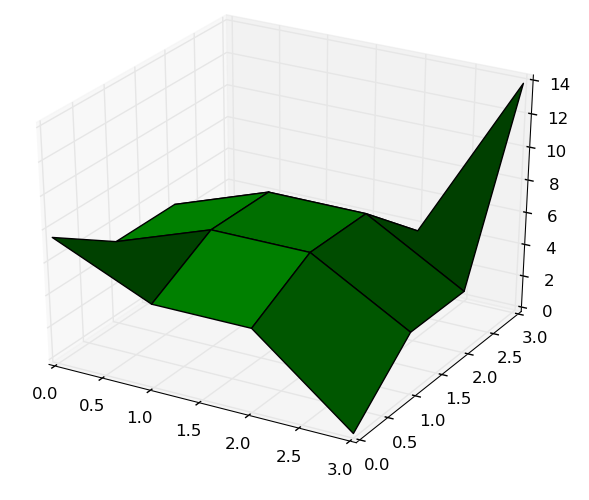
\includegraphics[scale=0.26]{realtests_real1.png} &
			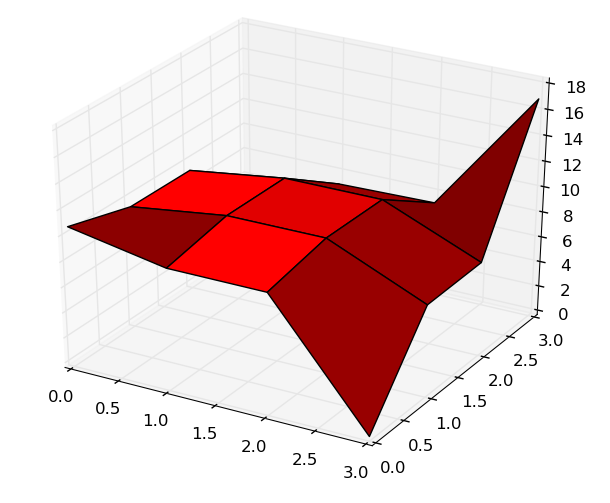
\includegraphics[scale=0.26]{realtests_sketchmin1.png} \\
			Exact codeviance & \texttt{SketchMin} algorithm \\
		\end{tabular}
	\end{center}
		
	\end{frame}
	
	\subsection{Randomly generated data}
	\begin{frame}{Generated data traces}
		\footnotesize
	
		\begin{block}{~}
		
		\center
		\begin{tabular}{c|c|c|c}
			size & interval $\left[0, u \right]$ & $\varepsilon$ & $\delta$ \\
			\hline
			$10~000$ & $u = 100$ & $0.1$ & $0.001$ \\
		\end{tabular}
		
		\end{block}
		
		\begin{center}
		\footnotesize
		
		\begin{tabular}{cc}
		
			\begin{tabular}{c}
				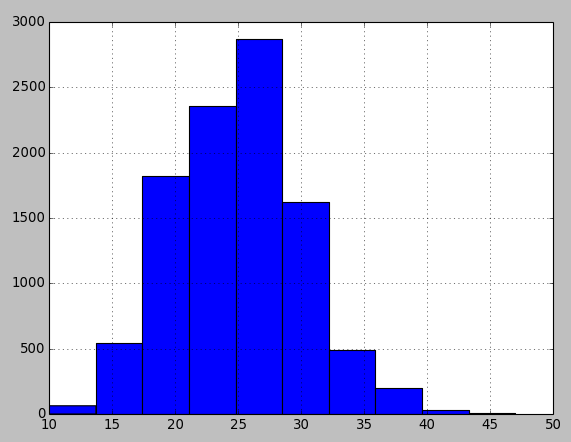
\includegraphics[scale=0.17]{poisson2.png}\\
				\text{\scriptsize Histogram of trace 7} \\
			\end{tabular}
			
		&

		
		\begin{tabular}{|c|c|c|}
			\hline
			 & Probabilistic laws & Parameters \\
			 \hline
			Trace 0 & Uniform & \\
			Trace 1 & Zipfian & $\alpha = 2$ \\
			Trace 2 & Zipfian & $\alpha = 3$ \\
			Trace 3 & Zipfian & $\alpha = 4$ \\
			Trace 4 & Zipfian & $\alpha = 5$ \\ 
			Trace 5 & Zipfian & $\alpha = 6$ \\
			Trace 6 & Poisson & $\lambda = u/(2)$ \\
			Trace 7 & Poisson & $\lambda = u/(2^2)$ \\
			Trace 8 & Poisson & $\lambda = u/(2^3)$ \\
			Trace 9 & Poisson & $\lambda = u/(2^4)$ \\
			Trace 10 & Poisson & $\lambda = u/(2^5)$ \\
			Trace 11 & Binomial & $p = 0.42$ \\
			Trace 12 & Negative Binomial & $p = 0.42$ \\
			\hline
		\end{tabular}
		
		\end{tabular}
		
		\end{center}
	\end{frame}
	
	\begin{frame}{Generated data traces}
	
	\begin{center}
		\begin{block}{Codeviance matrix of generated data traces}
		\end{block}
		\begin{tabular}{cc}
			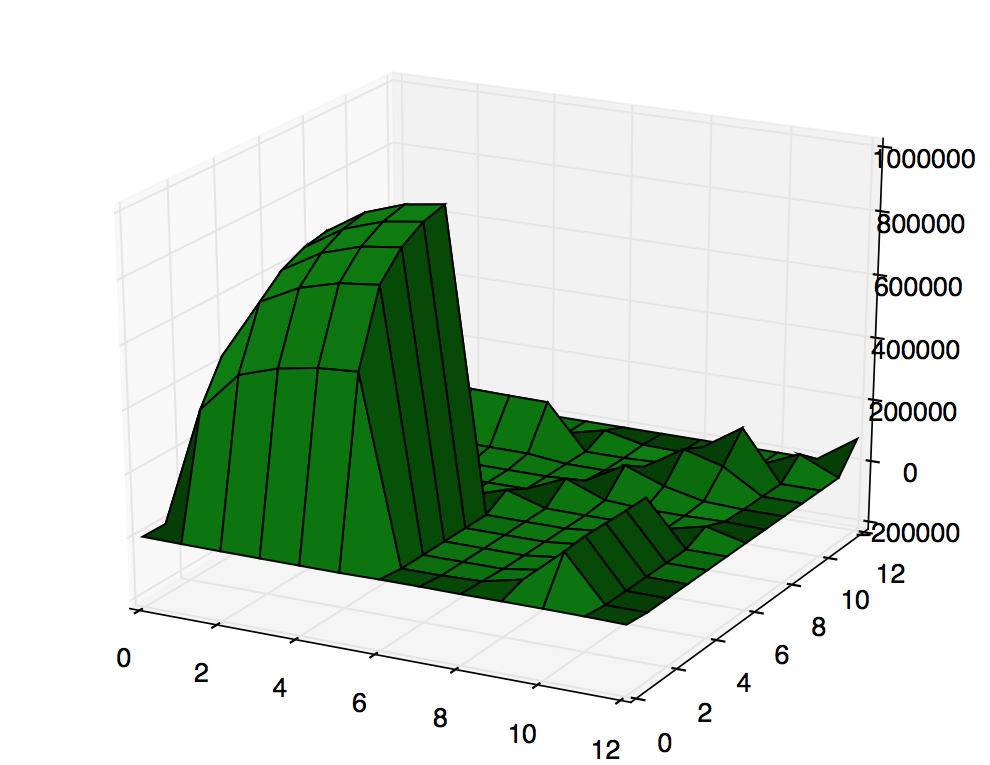
\includegraphics[scale=0.16]{generated_real.png} &
			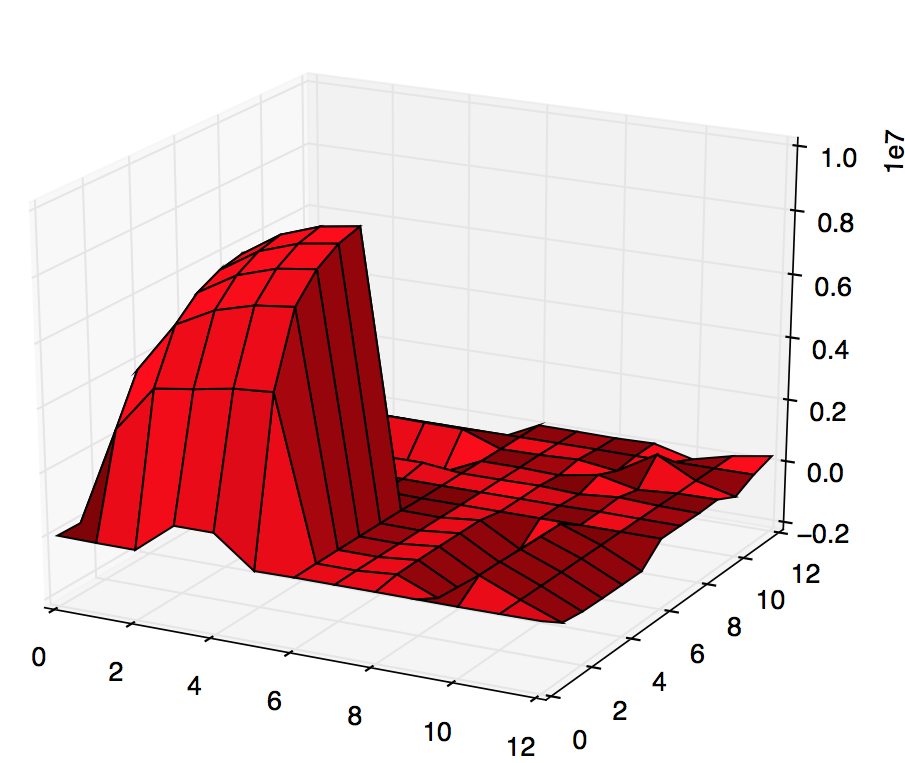
\includegraphics[scale=0.16]{generated_sk.png} \\
			Exact codeviance & \texttt{SketchMin} algorithm \\
		\end{tabular}
	\end{center}
		
	\end{frame}

\section*{Conclusion}

	\begin{frame}
		\begin{block}{}
			Algorithm results look the same as the exact entries, on a different scale. Can use the same method to detect attack on exact traces.
		\end{block}
		
		\begin{block}{Improvements}
			\begin{itemize}
				\item Work on flows of data traces instead of only one complete trace ;
				\item put in concurrency the hashing functions computations	;
				\item find a way of detecting attacks without false-detection.
			\end{itemize}
		\end{block}
	\end{frame}



\end{document}